



En el ejemplo TKTK, se define el conjunto de los números naturales $\nset =
\{0, 1, 2, 3, 4, \dots\}$, donde el siguiente de 0 es $s(0) = 1$, el
siguiente de 1 es $s(1) = 2$, y así sucesivamente. De esta forma, cada
número natural distinto del cero es definido como el siguiente de otro
número natural, y esto nos permite realizar la siguiente representación de
$\nset$:

$$ 0 \rightarrow s(0)\rightarrow s(s(0)) \rightarrow s(s(s(0))) \rightarrow
\cdots $$

\noindent es decir,

$$ 0 \rightarrow 1 \rightarrow 2 \rightarrow 3 \rightarrow \cdots $$

\noindent y describir la relación ``menor o igual que'', `$\leq$', en
$\nset$, mediante $n \leq m$, si y solo si hay un camino de flechas
$\rightarrow$ desde $n$ hasta $m$, en esa representación, o si $m$ y $n$ son
iguales. En esencia, lo que se establece es la ordenación de los números
naturales:

$$ 0 \leq 1 \leq 2 \leq 3 \leq \cdots $$

Este es el orden que usted conoce y al que está habituado, ya sea en $\nset$
o en cualquier otro conjunto numérico. En el álgebra abstracta, el concepto
de \emph{orden} es algo más abstracto y abarca a otras relaciones distintas
de la que acabamos de mencionar.

Definición. Relación de orden. Una relación $\rrel \subseteq U \times U$ se
denomina \emph{relación de orden} si posee las propiedades reflexiva,
antisimétrica y transitiva.

A veces, interesa hablar de un \emph{preorden}. Sería lo mismo que la de
orden solo que no haría falta que se cumpla la antisimétrica.

Muchas veces, nos permitimos ahorrarnos la palabra \emph{relación} y
simplemente dicimos que es un \emph{orden}.

Tal y como hemos explicado, al definir el concepto de \emph{orden} de esta
forma, encajarían aquí otras relaciones. Por ejemplo, una de estas sería la
de ``divide a'' en el conjunto $\nset^*$. Es fácil comprobar que cumple las
tres propiedades de la definición de relación de orden. Entonces, dados dos
elementos $a, b \in \nset^*$, si $a \mid b$, se puede decir que ``$a$
precede a $b$'', o, de forma algo más metafórica, que ``$a$ es menor que
$b$''.

% TODO Diagramas de Hasse.

La relación de orden $\rrel$ se dice que es de \emph{orden total} si posee
la propiedad

$$ \rrel^{-1} \cup \rrel = U \times U $$

\noindent o, dicho de otro modo,

$$ \forall x, y \in U. \ x \rrel y \ \text{o} \ y \rrel x $$

\noindent En caso contrario, será de \emph{orden parcial}.

Ejemplo. Orden entre subconjuntos. En la teoría de conjuntos, la relación
``contenido'', representada normalmente por `$\subseteq$', tiene la forma
siguiente

$$ \subseteq: \powset(U) \longrightarrow \powset(U) $$

\noindent y, para cualesquiera $A, B, C \in \powset(U)$, satisface las
propiedades que hacen que se trate de una relación de orden. Veámoslo.

\begin{itemize}
  \item Reflexiva. Se cumple $A \subseteq A$. Esto se demostró antes, TKTK.
  \item Antisimétrica. Si $A \subseteq B$ y $B \subseteq A$, entones $A =
    B$. Es la doble inclusión, que vimos que era cierta.
  \item Transitiva. Si $A \subseteq B$ y $B \subseteq C$, entonces $A
    \subseteq C$. Se deduce directamente de la definición de
    \emph{subconjunto}.
\end{itemize}

Es evidente que es un orden parcial, cosa que se podría demostrar con un
contraejemplo. Así, pues, sobre el conjunto $A = \{a, b, c\}$, para los
conjuntos $A_1 = \{a\}$ y $A_2 = \{b\}$, se tiene que $A_1 \not\subseteq
A_2$ y $A_2 \not\subseteq A_1$.

Ejemplo. Orden en $\nset$, $\zset$, $\qset$ y $\rset$. En cada uno de estos
conjuntos de números está definida la relación de orden habitual, `$\leq$',
``menor o igual que'', que es una relación de orden total. La definición del
orden en cada uno de estos conjuntos se verá en capítulos posteriores.

Cabe observar que, una vez establecida la relación orden $\leq$, se pueden
definir las relaciones habituales `$<$', ``estrictamente menor'', y `$>$',
``estrictamente mayor'', que no son relaciones de orden, puesto que no son
reflexivas, aunque sí son transitivas.

El par formado por un conjunto y una relación de orden definida sobre este
se denomina \emph{conjunto ordenado}.

Ya que nos movemos en conceptos muy genéricos y estamos usando una notación
que también se usa en un caso particular de relación de orden, es decir,
`$\leq$', es preferible pasar a usar otro símbolo con el que no exista
posibilidad de confusión. Lo más usual es hacer uso de `$\preceq$'. La forma
en que se leería algo como ``$a \preceq b$'' sería ``$a$ precede a $b$'' o
``$a$ antecede a $b$''.

También se utiliza indistintamente la notación $b \succeq a$, que se lee
``$b$ sucede a $a$'' o ``$b$ es posterior a $a$''. La notación $a \prec b$
se utiliza para indicar que $a \preceq b$ y $a \neq b$. Análogamente, para
$a \succ b$.

En todo conjunto ordenado, hay un tipo particular de subconjuntos a los que
se llama \emph{intervalos}.

Definición. Intervalos en un conunto ordenado. Dados un conjunto ordenado
$(U, \preceq)$ y los elementos $a, b \in U$ tales que $a \preceq b$, se
denominan \emph{intervalos} a cada uno de los conjuntos siguientes:

% TODO Explicación de cosas como a < x < b son como a < x y < < b.

intervalo abierto.

$$ (a, b) = \{x \in u \st a \prec x \prec b\} $$

intervalo cerrado.

$$ [a, b] = \{x \in u \st a \preceq x \preceq b\} $$

intervalos semiabiertos (o semicerrados también se les puede llamar).

\begin{align*}
  (a, b] &= \{x \in u \st a \prec x \preceq b\} \\
  [a, b) &= \{x \in u \st a \preceq x \prec b\} \\
\end{align*}

Obsérvese que, si $a = b$, entonces los intervalos $(a, b)$, $(a, b]$ y $[a,
b)$ son el conjunto vacío, $\emptyset$, mientras que el intervalo $[a, b]$
se reduce a un solo elemento: $a$, o $b$, si lo prefiere.

Ejemplo. Sea el conjunto ordenado $(\rset, \leq)$ donde la relación $\leq$
es el orden usual de $\rset$. La forma habitual de representar el conjunto
de los números reales es mediante los puntos de una recta, como en la
figura~\ref{fig:intervalo-r}. El lector está familiarizado con los
intervalos y semirrectas en la recta real que se ven como segmentos
continuos en dicha recta. La expresión $a\leq b$ se traduce gráficamente
como ``$a$ está a la izquierda de $b$ en la recta''.

\begin{figure}
  \centering
  \foreignlanguage{english}{
  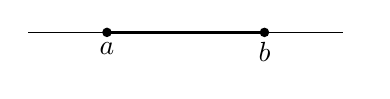
\begin{tikzpicture}
    % Línea principal
    \draw (-2, 0) -- (2, 0); % Eje real
    \draw[very thick] (-1, 0) -- (1, 0); % Intervalo cerrado [a, b]

    % Puntos en los extremos
    \filldraw (-1, 0) circle (1.5pt) node[below] {$a$};
    \filldraw (1, 0) circle (1.5pt) node[below] {$b$};

    % Etiqueta del eje real
    \node[below right] at (2,0) {$\rset$};
  \end{tikzpicture}
  }
  \caption{Intervalo cerrado $[a, b]$ en $\rset$.}
  \label{fig:intervalo-r}
\end{figure}

\noindent Sin embargo los intervalos pueden ser entendidos en el marco de
los otros conjntos numéricos ordenados, aunque se representen dentro de la
recta real.

El intervalo $[3, 6]$ en los números naturales, $\nset$, que denotaremos
como $[3, 6]_\nset$, es $[3, 6]_\nset = \{3, 4, 5, 6\}$. Por otro lado, se
tiene $(1, 2)_\nset = \emptyset$.

El intervalo $({-2}, 3]$ en los números enteros, $\zset$, es

$$ ({-2}, 3]_\zset = \{{-1}, 0, 1, 2, 3\} $$

\noindent y lo representamos gráficamente en la
figura~\ref{fig:intervalo-entero}. Otro ejemplo sería $(3, 4)_\zset =
\emptyset$.

\begin{figure}
  \centering
  \foreignlanguage{english}{
  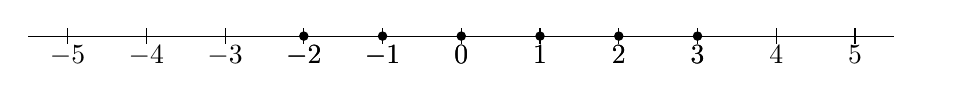
\begin{tikzpicture}
    % Línea principal (eje real)
    \draw (-5.5, 0) -- (5.5, 0);

    % Marcas de puntos en Z
    \foreach \x in {-5,...,5} {
      \draw (\x, 0.1) -- (\x, -0.1) node[below] at(\x, 0) {$\x$};
    }

    % Puntos en el intervalo
    \foreach \x in {-2,...,3} {
      \filldraw (\x, 0) circle (1.5pt) node[below] {${\x}$};
    }

    % Extremos del intervalo
    % TODO \draw (-2, 0) -- (\x, -0.1) node[below] at(\x, 0) {$\x$};

    % Etiqueta del eje real
    \node[below right] at (5.7, 0) {$\zset$};
  \end{tikzpicture}
  }
  \caption{Intervalo $[{-2}, 3]_\zset$.}%
  \label{fig:intervalo-entero}
\end{figure}

En general, los intervalos de $\nset$ y los de $\zset$ son puntos aislados
en la recta real $\rset$.

Cuando se desea hacer referencia al intervalo $({-3}, 4]_\qset$, en los
números racionales, $\qset$, se emplea la intersección de todo $\qset$ con
ese mismo intervalo pero de $\rset$, es decir,

$$ ({-3}, 4]_\qset = ({-3}, 4]_\rset \cap \qset $$

Definición. Intervalos iniciales y finales. Dado un conjunto ordenado $(U,
\succeq)$, los siguientes conjuntos también se denominan \emph{intervalos}.

\begin{center}
\begin{tabular}{l@{\quad}l}
  Intervalo inicial abierto:
    & $\displaystyle (\leftarrow, a) = \{x \in U \st x \prec a\}$ \\
  Intervalo final abierto:
    & $\displaystyle (a, \rightarrow) = \{x \in U \st a \prec x\}$ \\
  Intervalo inicial cerrado:
    & $\displaystyle (\leftarrow, a] = \{x \in U \st x \preceq a\}$ \\
  Intervalo final cerrado:
    & $\displaystyle [a, \rightarrow) = \{x \in U \st a \preceq x\}$ \\
\end{tabular}
\end{center}

Ejemplo. El lector está familiarizado con los intervalos iniciales y finales
(las semirrectas) en la recta real del ejemplo TKTK. Sin embargo, un
intervalo inicial o final puede ser entendido en el marco de los otros
conjuntos numéricos ordenados.

Por ejemplo, podríamos tener el siguiente intervalo inicial en los números
naturales: $(\leftarrow, 5)_\nset = [0, 4]_\nset = \{0, 1, 2, 3, 4\}$, y el
intervalo final en los enteros $[3, \rightarrow)_\nset = \{3, 4, 5,
\ldots\}$.

El intervalo inicial $(\leftarrow, 2)_\zset = \{\ldots, {-2}, {-1}, 0, 1\}$
en los números enteros, y el intervalo final $[3, \rightarrow)_\zset = \{3,
4, 5, \ldots\}$.

Los intervalos iniciales y finales en los números racionales, también se
escriben en función de los correspondientes intervalos en $\rset$:

\begin{align*}
  (\leftarrow, 2)_\qset = (\leftarrow, 2) \cap \qset \\
  (3, \rightarrow)_\qset = (3, \rightarrow) \cap \qset \\
\end{align*}

Orden lexicográfico en $\rset^2$. Basándonos en el orden usual de $\rset$,
definimos la relación siguiente de orden en $\rset^2$:

$$ (a, b) \leq_L (c, d) \ \text{si y solo si} \ (a < c) \ \text{o} \ (a = c
\ \text{y} \ b \leq d) $$

\noindent para $a, b, c, d \in \rset$.

Para representar un intervalo abierto o semiabierto, se tendría que hacer
uso de la versión estricta de esta relación, que sería:

$$ (a, b) <_L (c, d) \ \text{si y solo si} \ (a < c) \ \text{o} \ (a = c \
\text{y} \ b < d) $$

Podríamos representar, como en la figura~\ref{fig:orden-lexicografico-1}, el
intervalo inicial cerrado $(\leftarrow, (a, b)]_{\leq_L}$, que sería el área
sombreada de la izquierda junto a la semirrecta vertical continua izquierda,
incluyendo al punto $(a, b)$, y el intervalo final cerrado $[(c, d),
\rightarrow)_{\leq_L}$, correspondiente al área sombreada de la derecha y la
semirrecta vertical continua de la derecha, junto con el punto $(c, d)$.
Estos intervalos iniciales serían

\begin{align*}
  (\leftarrow, (a, b)]_{\leq_L}
    &= \{(x, y) \in \rset^2 \st (x, y) \leq _L (a, b)\} \\
  [(c, d), \rightarrow)_{\leq_L}
    &= \{(x, y) \in \rset^2 \st (c, d) \leq _L (x, y)\} \\
\end{align*}

Se trata de una relación de orden total ya que se puede comprobar que, dado
un punto $(a, b)$, entonces $(\leftarrow, (a, b)]_{\leq_L} \cup [((a, b),
\rightarrow)_{\leq_L} = \rset^2$, y, por tanto, cualquier punto $(x, y)$ del
plano está relacionado con un punto cualquiera $(a, b)$, ya sea mediante
$(x, y) \leq_L (a, b)$, o bien, $(a, b) \leq_L (x, y)$.

\begin{figure}
\centering
  \foreignlanguage{english}{
  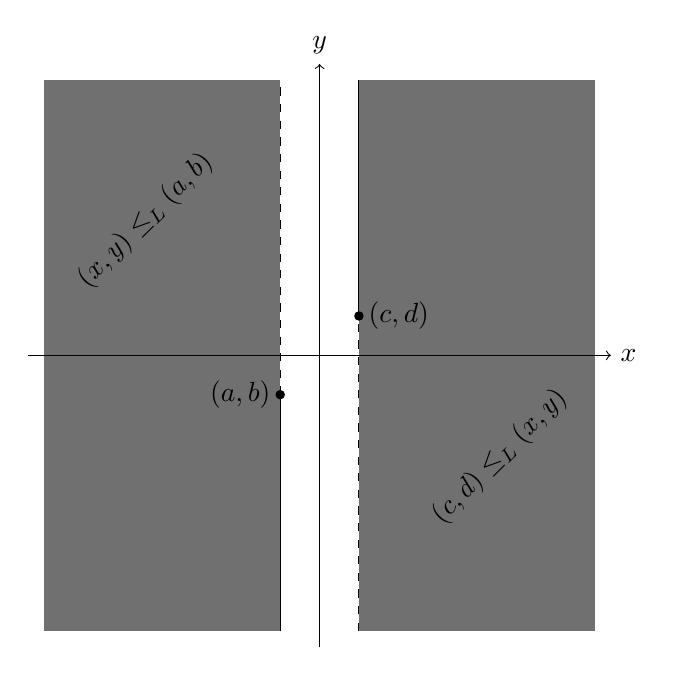
\begin{tikzpicture}[scale=1]

    % Áreas sombreadas
    \fill[gray!140, opacity=0.8] (-3.5, -3.5) rectangle (-0.5, 3.5);
    \fill[gray!140, opacity=0.8] (0.5, -3.5) rectangle (3.5, 3.5);

    % Ejes cartesianos
    \draw[->] (-3.7, 0) -- (3.7, 0) node[right] {$x$};
    \draw[->] (0, -3.7) -- (0, 3.7) node[above] {$y$};

    % Líneas verticales
    \draw (-0.5, -3.5) -- (-0.5, -0.5);
    \draw[dashed] (-0.5, -0.5) -- (-0.5, 3.5);

    \draw[dashed] (0.5, -3.5) -- (0.5, 0.5);
    \draw (0.5, 0.5) -- (0.5, 3.5);

    % Puntos en el plano
    \filldraw (-0.5, -0.5) circle (1.5pt) node[left] {$(a, b)$};
    \filldraw (0.5, 0.5) circle (1.5pt) node[right] {$(c, d)$};

    % Etiquetas de las relaciones
    \node[above, rotate= 45] at (-2, 1.5) {$(x, y) \leq_L (a, b)$};
    \node[above, rotate=45] at (2.5, -1.5) {$(c, d) \leq_L (x, y)$};

  \end{tikzpicture}
  }
  \caption{Intervalos $(\leftarrow, (a, b)]_{\leq_L}$ y $[(c,d),
    \to)_{\leq_L}$.}%
  \label{fig:orden-lexicografico-1}
\end{figure}

También, podríamos tener los intervalos inicial y final abiertos que, en
notación compacta, serían $(a, b) <_L (x, y) <_L (c, d)$. Su representación
gráfica la mostramos en la figura~\ref{fig:orden-lexicografico-2}.

\begin{figure}
\centering
  \foreignlanguage{english}{
  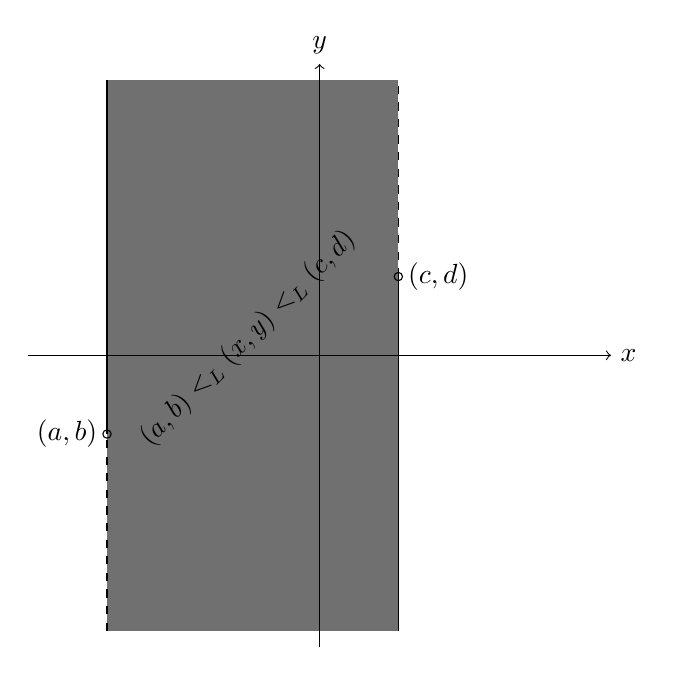
\begin{tikzpicture}[scale=1]

    % Áreas sombreadas
    \fill[gray!140, opacity=0.8] (-2.7, -3.5) rectangle (1, 3.5);

    % Ejes cartesianos
    \draw[->] (-3.7, 0) -- (3.7, 0) node[right] {$x$};
    \draw[->] (0, -3.7) -- (0, 3.7) node[above] {$y$};

    % Líneas verticales
    \draw[dashed] (-2.7, -3.5) -- (-2.7, -1);
    \draw (-2.7, -1) -- (-2.7, 3.5);

    \draw (1, -3.5) -- (1, 1);
    \draw[dashed] (1, 1) -- (1, 3.5);

    % Puntos en el plano
    \draw (-2.7, -1) circle (1.5pt) node[left] {$(a, b)$};
    \draw (1, 1) circle (1.5pt) node[right] {$(c, d)$};

    % Etiquetas de las relaciones
    \node[above, rotate= 45] at (-0.7, 0)
      {$(a, b) <_L (x, y) <_L (c, d)$};

  \end{tikzpicture}
  }
  \caption{Intervalo $((a, b), (c, d))_{\leq_L}$.}%
  \label{fig:orden-lexicografico-2}
\end{figure}

Esta relación de orden la llaman \emph{lexicográfica} porque viene de que el
orden es análogo al que se utiliza para disponer las palabras en un
diccionario.

Ejemplo. Orden producto en $\rset^2$. Se define en $\rset^2$, componente a
componente, el siguiente orden

$$ (a, b) \leq_P (c, d) \ \text{si y solo si} \ a \leq c \ \text{y} \ b \leq
d $$

\noindent entendiendo que ese `$\leq$' es el orden usual de los números
reales. Su versión estricta, para poder hacer uso de intervalos abiertos o
semiabiertos, sería

$$ (a, b) \leq_P (c, d) \ \text{si y solo si} \ a < c \ \text{y} \ b < d $$

La relación producto es un orden parcial en $\rset^2$ que en economía suelen
llamar \emph{orden de Pareto}. En general, cuando se tienen dos espacios
ordenados, el orden producto es el orden que se define en el producto
cartesiano componente a componente.

En las figuras~\ref{fig:orden-pareto-1} y~\ref{fig:orden-pareto-2},
mostramos las representaciones de intervalos según el orden producto.
Advierta que en la primera se ve claramente que el orden producto no es
total, ya que dado un punto $(a, b)$, se tiene que $\rset^2 \neq
(\leftarrow, (a, b)]_{\leq_P} \cup [(a, b), \rightarrow)_{\leq_P}$. De
hecho, si $a \neq b$, los puntos $(a, b)$ y $(b, a)$ no son comparables, es
decir, ni $(b, a) \leq_P (a, b)$ ni $(a, b) \leq_P (b, a)$.

\begin{figure}
\centering
  \foreignlanguage{english}{
  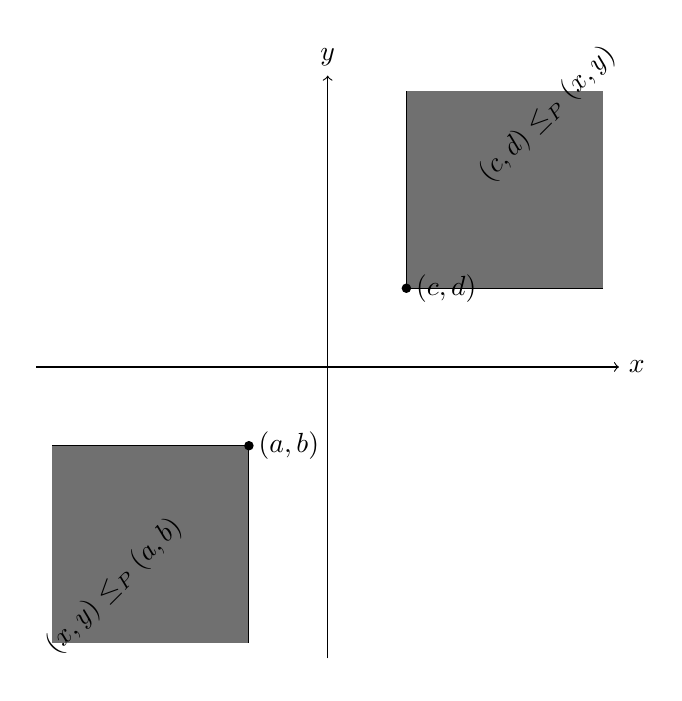
\begin{tikzpicture}[scale=1]

    % Áreas sombreadas
    \fill[gray!140, opacity=0.8] (-3.5, -3.5) rectangle (-1, -1);
    \fill[gray!140, opacity=0.8] (1, 1) rectangle (3.5, 3.5);

    % Ejes cartesianos
    \draw[->] (-3.7, 0) -- (3.7, 0) node[right] {$x$};
    \draw[->] (0, -3.7) -- (0, 3.7) node[above] {$y$};

    % Líneas
    \draw (-1, -3.5) -- (-1, -1) -- (-3.5, -1);
    \draw (3.5, 1) -- (1, 1) -- (1, 3.5);

    % Puntos en el plano
    \filldraw (-1, -1) circle (1.5pt) node[right] {$(a, b)$};
    \filldraw (1, 1) circle (1.5pt) node[right] {$(c, d)$};

    % Etiquetas de las relaciones
    \node[above, rotate= 45] at (-2.5, -3) {$(x, y) \leq_P (a, b)$};
    \node[above, rotate=45] at (3, 3) {$(c, d) \leq_P (x, y)$};

  \end{tikzpicture}
  }
  \caption{Intervalos $(\leftarrow, (a, b)]_{\leq_P}$ y $[(c, d),
    \rightarrow)_{\leq_P}$.}%
  \label{fig:orden-pareto-1}
\end{figure}

\begin{figure}
\centering
  \foreignlanguage{english}{
  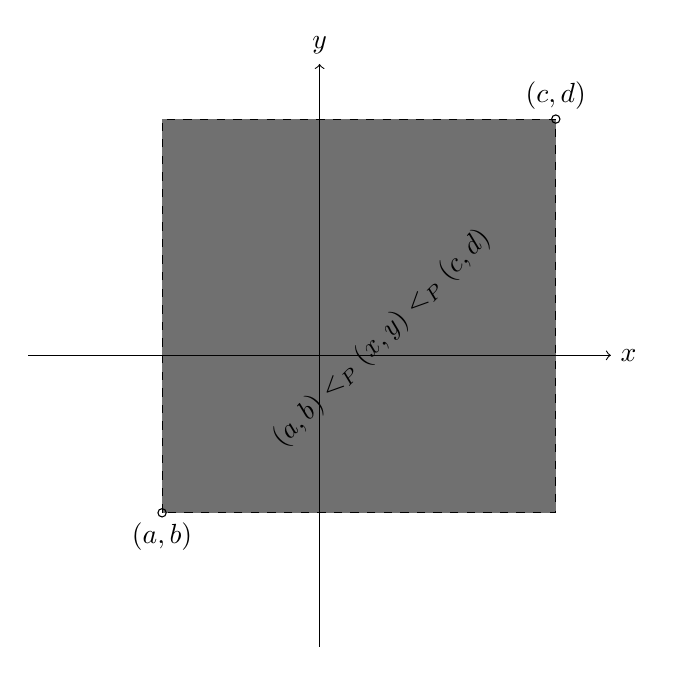
\begin{tikzpicture}[scale=1]

    % Áreas sombreadas
    \fill[gray!140, opacity=0.8] (-2, -2) rectangle (3, 3);

    % Ejes cartesianos
    \draw[->] (-3.7, 0) -- (3.7, 0) node[right] {$x$};
    \draw[->] (0, -3.7) -- (0, 3.7) node[above] {$y$};

    % Líneas
    \draw[dashed] (-2, -2) -- (-2, 3) -- (3, 3) -- (3, -2) -- (-2, -2);

    % Puntos en el plano
    \draw (-2, -2) circle (1.5pt) node[below] {$(a, b)$};
    \draw (3, 3) circle (1.5pt) node[above] {$(c, d)$};

    % Etiquetas de las relaciones
    \node[above, rotate= 45] at (1, 0)
      {$(a, b) <_P (x, y) <_P (c, d)$};

  \end{tikzpicture}
  }
  \caption{Intervalo $((a, b), (c, d))_{\leq_P}$.}%
  \label{fig:orden-pareto-2}
\end{figure}

% TODO Quizás, crear una (sub)sección sobre acotación.

Definición. Cotas de un subconjunto $A$. Dados un conjunto ordenado $(U,
 \preceq)$ y un subconjunto $A \subseteq U$, se denomina \emph{cota
 superior} del conjunto $A$ a un elemento de $U$ que suceda a todo elemento
 de $A$, y será una \emph{cota inferior} de $A$ todo elemento de $U$ que
 preceda a todo elemento de $A$.

 Esto mismo se podría expresar haciendo más uso de simbología. Una cota
superior de $A$ es cualquier elemento $u \in U$ que cumple que $\forall x
\in A. \ x \preceq u$, mientras que, una cota inferior de $A$ es cualquier
elemento $d \in U$ que cumple que $\forall x \in A. \ d \preceq x$.

Si, para un conjunto $A$, existe una cota superior en este, se dice que el
conjunto $A$ está acotado superiormente. Análogamente, si para un conjunto
$A$ se tiene una cota inferior, se dirá que $A$ está acotado inferiormente.
Se dice que un conjunto está \emph{acotado} si está acotado superiormente e
inferiormente.

Observación. En un conjunto ordenado $(U, \preceq)$ se tiene que un conjunto
$A \subseteq U$ está acotado si y solo si existen dos elementos $a, b \in U$
tales que $A$ está contenido en el intervalo $[a, b]_{\preceq}$.

Definición. Máximo y mínimo de un conjunto $A$. Dados un conjunto ordenado
$(U, \preceq)$ y un subconjunto $A \subseteq U$, se denomina \emph{máximo}
del conjunto $A$, denotado por $\mmax(A)$, a una cota superior de $A$ que
pertenezca a $A$, mientras que será un \emph{mínimo} de $A$, que
representaremos por $\mmin(A)$, una cota inferior de $A$ que pertenezca a
$A$.

Se podrían dar estas definiciones haciendo más uso de la simbología. Un
máximo de $A$ es todo elemento $m \in A$ tal que $\forall x \in A. \ x
\preceq m$, mientras que un mínimo de $A$ es todo elemento $m \in A$ tal que
$\forall x \in A. \ m \preceq x$.

Definición. Supremo e ínfimo de un conjunto $A$. Dados un conjunto ordenado
$(U, \preceq)$ y un subconjunto $A \subseteq U$, llamamos \emph{supremo} de
$A$, representado por $\msup(A)$, a toda cota superior de $A$ que preceda a
las demás. Análogamente, será \emph{ínfimo} de $A$, representado por
$\minf(A)$, toda cota inferior de $A$ que suceda a las demás.

Se podrían definir haciendo un mayor uso de la simbología. El supremo de $A$
es una cota superior $s \in U$ de $A$ tal que $s \preceq u$ para toda cota
superior $u$ de $A$, mientras que el ínfimo de $A$ es una cota inferior $i
\in U$ de $A$ tal que $d \preceq i$ para toda cota superior $d$ de $A$.

Observaciones. En un conjunto ordenado $(U, \preceq)$, se tiene que el
ínfimo de un conjunto $A$ es el máximo del conjunto de las cotas inferiores
de $A$, y el supremo de $A$ es el mínimo del conjunto de las cotas
superiores de $A$.

Proposición. Si un conjunto posee máximo, entonces posee supremo, y, además,
$\msup(A) = \mmax(A)$. Análogamente. si un conjunto posee mínimo, entonces
posee ínfimo, e $\minf(A) = \mmin(A)$.

Para demostrarlo, es fácil ver que se deduce de forma directa de la
definición de TKTK.

% TODO Todo esto habrá que trabajarlo y consultarlo en otras fuentes, pues
% parecen proposiciones importantes pero que menciona muy de pasada.

De aquí podemos deducir su condicional contrarrecíproca, que también tiene
su utilidad. Es la siguiente:

Proposición. Si $\msup(A) \notin A$, entonces no existe $\mmax(A)$.

Tal como veremos ahora, se dan ciertas propiedades sobre la existencia de
los elementos que acabamos de ver. Concretamente, aunque no hemos querido
especificarlo en la definición, tanto el máximo, mínimo, supremo e ínfimo,
en caso de existir, son únicos. Lo vemos en la proposición siguiente.

Proposición. Dados un conjunto ordenado $(U, \preceq)$ y un subconjunto $A$
de $U$, $A \subseteq U$, se tiene

\begin{itemize}
  \item Si existe el máximo del conjunto $A$, entonces este es único. Lo
    mismo sucede para el mínimo.
  \item Si existe el supremo de $A$, entonces este es único. Lo mismo sucede
    para el ínfimo.
  \item Si existe el supremo $s$ del conjunto $A$ y $s \in A$, entonces $s$
    es el máximo de $A$.
  \item Si existe el ínfimo $i$ del conjunto $A$ e $i \in A$, entonces $i$
    es el mínimo de $A$.
\end{itemize}

Demostración. Veamos las demostraciones de algunas de estas proposiciones.

Para la primera, sobre el máximo, sería lo siguiente. Suponemos que existen
$m, m' \in A$ tales que para cualquier $x \in A$ se cumple que $x \preceq m$
y $x \preceq m'$. En particular, se cumple, según el punto de vista, que
tanto $m' \preceq m$ como $m \preceq m'$. Por tanto, se tiene directamente
de la propiedad antisimétrica que se debe cumplir en toda relación de orden,
que $m = m'$. Ocurre lo mismo con el mínimo.

Para la del supremo, la demostración sería muy parecida. El supremo sería
una cota superior que precede a todas las demás. Supondríamos la existencia
de dos supremos de $A$: $s$ y $s'$. Según los dos puntos de vista, se
tendría que $s \preceq s'$ y $s' \preceq s$, con lo que, gracias a la
propiedad antisimétrica, se tiene que $s = s'$. Para el caso del ínfimo, se
seguiría un razonamiento análogo.

Debido a las afirmaciones anteriores, se puede decir, más cómodamente, que
el supremo de $A$ es la menor de sus cotas superiores, y, el ínfimo, la
mayor de las inferiores. Ojo, ``menor'' y ``mayor'' en el sentido del orden
(es decir, la relación de orden) que estamos tratando; no tiene por qué ser
el orden al que estamos acostumbrados.

Ejemplo. En el conjunto de los números naturales $\nset^*$, véase el ejemplo
TKTK, se define la relación ``divide a'' mediante

$$ n \mid m \ \text{si y solo si} \ \exists k \in \nset^* \ \text{tal que} \
m = kn $$

\noindent para $m, n \in \nset^*$. Es una relación de orden, puesto que,
para cualesquiera $m, n, h \in \nset^*$, se cumple:

\begin{itemize}
  \item Reflexiva, pues $n = 1n$.
  \item Antisimétrica, pues, si $m = kn$ y $n = k'm$, para unos $k, k' \in
    \nset^*$, entonces $n = k'kn$. Luego $k'k = 1$, de donde $k' = k = 1$.
  \item Transitiva pues, si $n \mid m$ y $m \mid h$, entonces $m = kn$ y $h
    = k'm$, para unos $k, k' \in \nset^*$, y, por tanto, $h = k'kn$, con lo
    que $n \mid h$.
\end{itemize}

Esta relación no es de orden total, cosa que se podría demostrar con un
contraejemplo: Los números 2 y 3 no están relacionados en ninguno de los
sentidos, es decir, $2 \nmid 3$ y $3 \nmid 2$.

El conjunto $A = \{2, 4, 6\}$ tiene como cota superior cualquier número que
sea divisible por 4, y 6, ya que, al ser divisible por uno cualquiera de
estos, también será divisible entre 2, automáticamente. En cuanto al
supremo, se tiene que $\msup(A) = 12$ pues el mínimo común múltiplo de esos
dos números es 12. Además, no existe máximo puesto que de existir debería
ser 12, pero $12 \notin A$. Las cotas inferiores son los números 1 y 2.
Además, $\mmin(A) = 2 = \minf(A)$.

Ejemplo. En el conjunto ordenado de los números racionales, $\qset$, se
considera el conjunto

$$ A = \{x \in \qset \st x^2 < 2\} $$

Se deduce fácilmente que ${-\sqrt{2}} < x < \sqrt{2}$ para $x \in \qset$, o,
lo que es lo mismo, $A = [{-\sqrt{2}}, \sqrt{2}] \cap \qset$. Entonces, una
cota inferior de $A$ en $\qset$ es ${-2}$, mientras que una superior es 2.
Ahora bien, no existe ni supremo ni ínfimo de $A$ en el conjunto $\qset$.
Esto se verá en detalle posteriormente, véase el ejemplo TKTK. Si se tratase
de un intervalo de $\rset$, es decir, $[{-\sqrt{2}}, \sqrt{2}]$, se tendría
que $\msup(A) = \sqrt{2}$ y $\minf(A) = {-\sqrt{2}}$. Tampoco existen
$\mmax(A)$ ni $\mmin(A)$ en $A$.

Propiedad del buen orden. Se dice que un conjunto ordenado $(U, \preceq)$ es
un conjunto \emph{bien ordenado}, o que la relación $\preceq$ es una buena
ordenación, si cualquier subconjunto no vacío posee mínimo.

En caso de existir, al elemento mínimo de cada subconjunto $A$ también se
denomina \emph{primer elemento} de $A$.

Concretamente, la propiedad de buena ordenación se cumple en el conjunto de
los números naturales, $\nset$. A esta la suelen llamar el Principio de
Buena Ordenación de $\nset$. Por tanto, tal y como veremos en un capítulo
posterior, todo conjunto no vacío de números naturales tiene mínimo.

Tal y como sucedía en el ejemplo anterior, en un conjunto ordenado un
subconjunto acotado puede no tener supremo ni ínfimo.

Ejemplo. El conjunto $A = \{(x, y) \in \rset^2 \st 1 \leq x \leq 2\}$ está
acotado superiormente en $\rset^2$ dotado del orden lexicográfico. Así, por
ejemplo, una cota superior sería $(3, {-7})$. Para hallar el supremo, es
bastante evidente que la primera coordenada sería el 2, pero la segunda no
tiene límite por debajo, con lo que podemos afirmar que dicho conjunto no
tiene supremo.

Por otro lado, una cota inferior sería el $(0, 0)$. Al tener cotas
superiores e inferiores, se trata de un conjunto acotado. Con el ínfimo,
sucedería algo similar al supremo. TKTK. No tiene.

Propiedad del supremo. Se dice que un conjunto ordenado $(U, \preceq)$ cuple
la propiedad del supremo si y solo si cualquier subconjunto no vacío $A$
acotado superiormente posee supremo.

La propiedad del supremo es una propiedad característica del orden de los
números reales, orden continuo. que se conoce como axioma del supremo de
$\rset$: Todo conjunto no vacío de números reales acotado superiormente
tiene supremo.

Advierta que esto no quiere decir que tenga máximo.

Ejemplo. Sea el conjunto $A = \{(x, y) \in \rset^2 \st 1 \leq x \leq 2, \ 1
\leq y < 2\}$ en el conjunto ordenado $\rset^2$ dotado del orden
lexicográfico, es decir, el conjunto ordenado $(\rset, \leq_L)$. Determine,
para $A$, las cotas inferiores y superiores, supremo e ínfimo y máximo y
mínimo.

Solución. Tal y como se puede ver en su representación gráfica, en la
figura~\ref{fig:orden-cotas-lexi-1}, una cota superior de $A$ es cualquier
punto del intervalo final cerrado $[(2, 2), \rightarrow)_L$, es decir,
cualquier $(x, y)$ con $2 < x$, que corresponde al área sombreada de la
derecha, o $(2, y)$ con $2 \leq y$, que es la semirrecta vertical desde el
punto $(2, 2)$, sin incluirlo, hacia ariba.

El supremo de $A$ es $\msupL (A) = (2, 2)$. El conjunto $A$ no posee máximo,
debido a que aparece una desigualdad estricta, $1 \leq y < 2$, en una de las
condiciones en la definición del conjunto $A$. TKTK.

Una cota inferior de $A$ es cualquier punto del intervalo inicial
$(\leftarrow, (1, 1)]_L$, es decir, cualquier $(x, y)$ con $x < 1$, que
corresponde con el área sombreada de la izquierda, o $(1, y)$ con $y \leq
1$, que es la semirrecta vertical hacia abajo desde en el punto $(1, 1)$,
incluido este. El ínfimo de $A$ es $\minfL(A) = (1, 1)$. Como el conjunto
$A$ contiene al punto $(1, 1)$, entonces $\mminL(A) = (1, 1)$.

\begin{figure}
\centering
  \foreignlanguage{english}{
  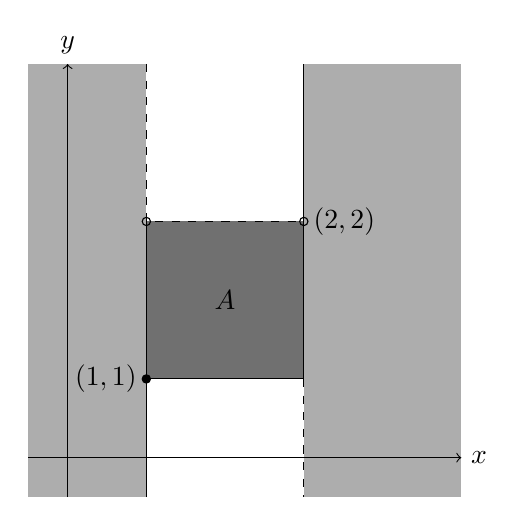
\begin{tikzpicture}[scale=1]

    % Áreas sombreadas
    \fill[gray!140, opacity=0.8] (1, 1) rectangle (3, 3);
    \fill[gray!80, opacity=0.8] (-0.5, -0.5) rectangle (1, 5);
    \fill[gray!80, opacity=0.8] (3, -0.5) rectangle (5, 5);

    % Ejes cartesianos
    \draw[->] (-0.5, 0) -- (5, 0) node[right] {$x$};
    \draw[->] (0, -0.5) -- (0, 5) node[above] {$y$};

    % Líneas
    \draw (1, 3) -- (1, 1) -- (3, 1) -- (3, 5);
    \draw (1, -0.5) -- (1, 1);
    \draw[dashed] (1, 5) -- (1, 3) -- (3, 3);
    \draw[dashed] (3, 1) -- (3, -0.5);

    % Puntos
    \filldraw (1, 1) circle (1.5pt) node[left] {$(1, 1)$};
    \draw (3, 3) circle (1.5pt) node[right] {$(2, 2)$};
    \draw (1, 3) circle (1.5pt);

    % Etiquetas
    \node at (2, 2) {$A$};

  \end{tikzpicture}
  }
  \caption{Cotas lexicográficas del conjunto $A \subseteq \rset^2$.}
  \label{fig:orden-cotas-lexi-1}
\end{figure}

Ejercicio. Sea el mismo conjunto $A = \{(x, y) \in \rset^2 \st 1 \leq x \leq
2, \ 1 \leq y < 2\}$ del ejercicio anterior, solo que ahora consideramos el
conjunto ordenado $(\rset, \leq_P)$, es decir, con el orden producto.
Determine, cotas inferiores y superiores, supremo. ínfimo, máximo y mínimo
de $A$.

Solución. Tal y como puede ver en la figura~\ref{fig:orden-cotas-prod-1},
una cota superior de $A$ es cualquier punto del intervalo final $[(2, 2),
\rightarrow)_P$, es decir, cualquier $(x, y)$ con $2 \leq x$ y $2 \leq y$,
que en la figura será el área sombreada superior derecha. El supremo de $A$
es $\msupP(A) = (2, 2)$. El conjunto $A$ no posee máximo puesto que $(2, 2)
\notin A$.

Una cota inferior de $A$ es cualquier punto del intervalo inicial
$(\leftarrow, (1, 1)]_P$, es decir, cualquier $(x, y)$ con $x \leq 1$ e $y
\leq 1$. El ínfimo de $A$ es $\minfP(A) = (1, 1)$. Como el conjunto $A$
contiene al punto $(1, 1)$, entonces $\mminP(A) = (1, 1)$.

\begin{figure}
\centering
  \foreignlanguage{english}{
  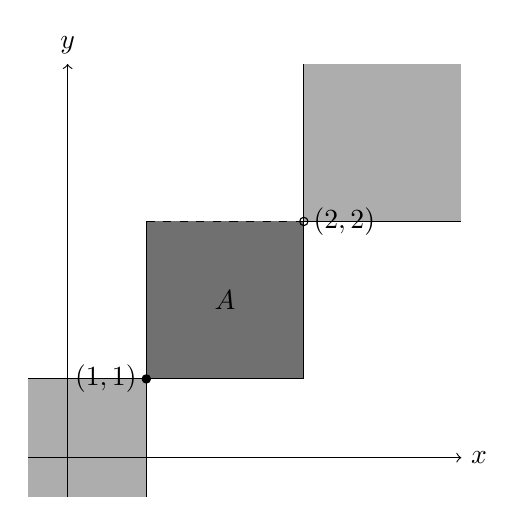
\begin{tikzpicture}[scale=1]

    % Áreas sombreadas
    \fill[gray!140, opacity=0.8] (1, 1) rectangle (3, 3);
    \fill[gray!80, opacity=0.8] (-0.5, -0.5) rectangle (1, 1);
    \fill[gray!80, opacity=0.8] (3, 3) rectangle (5, 5);

    % Ejes cartesianos
    \draw[->] (-0.5, 0) -- (5, 0) node[right] {$x$};
    \draw[->] (0, -0.5) -- (0, 5) node[above] {$y$};

    % Líneas
    \draw[dashed] (1, 3) -- (3, 3);
    \draw (1, -0.5) -- (1, 3);
    \draw (-0.5, 1) -- (3, 1) -- (3, 5);
    \draw (3, 3) -- (5, 3);

    % Puntos
    \filldraw (1, 1) circle (1.5pt) node[left] {$(1, 1)$};
    \draw (3, 3) circle (1.5pt) node[right] {$(2, 2)$};

    % Etiquetas
    \node at (2, 2) {$A$};

  \end{tikzpicture}
  }
  \caption{Cotas lexicográficas del conjunto $A \subseteq \rset^2$.}
  \label{fig:orden-cotas-prod-1}
\end{figure}

Ejemplo. Sea el conjunto $B$ constituido por la arista inferior y la arista
izquierda del cuadrado que representa al conjunto $A$ de los dos ejercicios
anteriores, es decir,

$$ B = \{(x, y) \in \rset^2 \st (1 \leq x \leq 2, \ \text{e} \ y = 1) \
\text{o} \ (1 \leq y \leq 2 \ \text{y} \ x = 1)\} $$

\noindent Resulta que, para el orden producto, $\leq_P$, el conjunto de las
cotas superiores de $B$ es el conjunto de las cotas superiores de $A$, y el
conjunto de las cotas inferiores de $B$ es el conjunto de las cotas
inferiores de $A$.

El supremo de $B$ es $\msupP(B) = (2, 2)$, y no existe $\mmaxP(B)$. Además,
$\minfP(B) = (1, 1) = \mminP(B)$. Fíjese en que el punto $(1,5, 3)$ no sería
una cota superior de $B$ por el orden producto. De hecho, al no tratarse de
un orden parcial, hay puntos que no están relacionados.

% TODO Explicarlo mejor.

Respecto al orden lexicográfico, el supremo de $B$ es $\msupL(B) = (2,
1)$, y, como $(2, 1) \in B$, resulta que es máximo. El ínfimo de $B$ es
$\minfL(A) = (1, 1)$ y, además, $\mminL(B) = (1, 1)$.

Ahora, vamos a presentar unos conceptos que serían como el de \emph{máximo}
y \emph{mínimo} solo que con un orden no estricto. Recuerde que, dada una
relación de orden $\preceq$, su correspondiente orden estricto se
representaría por $\prec$ y lo definiríamos como

$$ a \prec b \ \text{si y solo si} \ a \preceq b \ \text{y} \ a \neq b $$

Definición. Dados un conjunto ordenado $(U, \preceq)$ y un subconjunto $A$
de $U$, $A \subseteq U$, se define el \emph{elemento maximal} (\emph{maximal
element}) del conjunto $A$ como un elemento $M \in A$ tal que

$$ \not\exists x \in A. \ M \prec x $$

De forma dual, se tiene al \emph{elemento minimal} (\emph{minimal element})
del conjunto $A$ como un elemento $m \in A$ tal que

$$ \not\exists x \in A. \ x \prec m $$

A estos elementos, muchas veces se les llama simplemente \emph{maximal} y
\emph{minimal}, pues se sobrentiende que se trata de elementos.

En realidad, estos elementos se definen sobre conjuntos con preorden, pero
tampoco es algo que vayamos a estudiar en profundidad en esta asginatura.

Observación. Si el orden de $U$ es total, los conceptos de maximal y máximo
coinciden, así como los de minimal y mínimo. En general, los elementos
maximales y los minimales de un conjunto no tienen por qué ser únicos, como
se muestra en el el ejemplo siguiente. Sin embargo, si un conjunto tiene
elemento máximo, entonces solo hay un elemento maximal, y este coincidirá
con su máximo. Análogamente, para el mínimo. Es decir, si un conjunto tiene
un elemento mínimo, entonces solo hay un minimal, y este coincidirá con su
mínimo.

Ejemplo. En el conjunto ordenado del ejemplo TKTK, $(\nset^*, |)$, se
considera el conjunto $A = \{2, 3, 4, 5, 6, 7, 8, 9, 10\}$. Querríamos
hallar los elementos máximo, mínimo, maximal y minimal.

Si se fija, no tiene máximo, ya que no existe un $M \in A$ tal que para todo
$x \in A$ se dé $x \nmid M$. Se haría comprobándolo para todos y cada uno de
los elementos de $A$.

Por cierto, el orden es parcial, como es fácil ver con un contraejemplo.
Así, se tiene que $2 \nmid 3$ y $3 \nmid 2$.

Tampoco tiene mínimo, cosa que se comprobaría de forma análoga. Se puede
comprobar que no existe un $m \in A$ tal que, para todo $x \in A$, se dé $m
\mid x$. Se tendría que comprobar para todos los elementos de $A$.

Veamos ahora si tiene elementos maximales. Tenemos que averiguar si existe
algún $M \in A$ para el que no existe un $x \in A$ con el que se dan $M \neq
x$ y $M \mid x$. Con esta condición, se tiene que, por ejemplo, el 2 no lo
es, ya que divide al 4, entre otros. El 3, tampoco, porque al menos divide
al 6. Así, tendríamos que los elementos maximales de $A$ son $\{6, 7, 8, 9,
10\}$. Por otro lado, los minimales son $\{2, 3, 5, 7\}$, pues, por ejemplo,
el 2 no tiene en $A$ a ningún elemento que le divida y que no sea 2; con el
3, lo mismo; el 4 sí, pues $2 \mid 4$. Etc.

Aunque no nos lo han preguntado, una cota superior sería, por ejemplo, el
producto de todos ellos.

Ejercicio. Determine cotas, supremo ínfimo, máximo. mínimo, maximales y
minimales del conjunto

$$ A = \{(x,y) \in \rset^2 \st 0 \leq x, \ 0 \leq y, \ x + y \leq 1\} $$

\noindent para el orden lexicográfico y para el orden producto.

Solución. El conjunto $A$ es el conjunto de puntos del triángulo de vértices
$(0, 0)$, $(1, 0)$ y $(0, 1)$ y de su interior. Advierta que esas
condiciones se unen mediante conjunciones. Las dos primeras nos harían
descartar los cuadrantes 2, 3 y 4. Con la otra, nos quedamos con ese
tríángulo.

\begin{figure}
\centering
  \foreignlanguage{english}{
  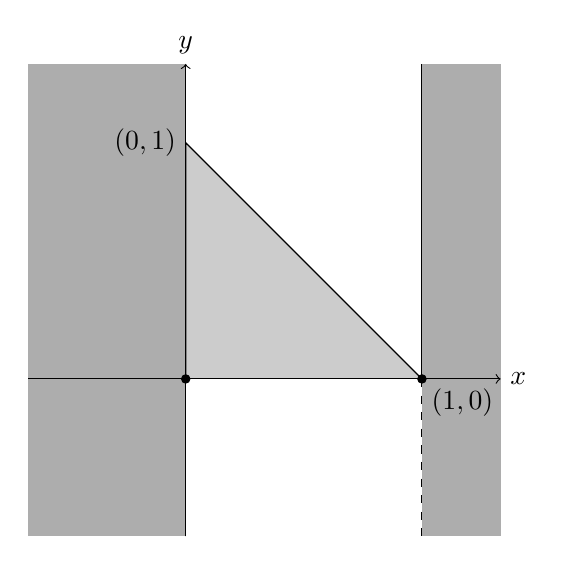
\begin{tikzpicture}[scale=1]

    % Áreas sombreadas
    \fill[gray!80, opacity=0.8] (-2, -2) rectangle (0, 4);
    \fill[gray!80, opacity=0.8] (3, -2) rectangle (4, 4);
    %\fill[gray!140, opacity=0.8] (1, 1) triangle (2, 2);
    % Triángulo
    \fill[gray!50, opacity=0.8] (0, 0) -- (3, 0) -- (0, 3) -- cycle;

    % Ejes cartesianos
    \draw[->] (-2, 0) -- (4, 0) node[right] {$x$};
    \draw[->] (0, -2) -- (0, 4) node[above] {$y$};

    % Líneas
    \draw (0, -2) -- (0, 0) -- (3, 0) -- (3, 4);
    \draw (0, 0) -- (0, 3) -- (3, 0);
    \draw[dashed] (0, 0) -- (0, 4);
    \draw[dashed] (3, 0) -- (3, -2);

    % Puntos
    \filldraw (0, 0) circle (1.5pt);
    \filldraw (3, 0) circle (1.5pt) node[anchor=north west] {$(1, 0)$};

    % Etiquetas
    \node[left] at (0, 3) {$(0, 1)$};

  \end{tikzpicture}
  }
  \caption{Cotas lexicográficas del conjunto $A \subseteq \rset^2$.}
  \label{fig:}
\end{figure}

Primera parte. TKTK. Con $\rset^2$ dotado del orden lexicográfico
tenemos que: 

Una cota superior de $A$ es cualquier punto $(x, y)$ tal que $1 < x$ o un
punto $(1, y)$ con $0 \leq y$, es decir, un punto del intervalo final
$\left[(1, 0), \to\right)_L$. Esto no quiere decir que sean las únicas. Por
ejemplo, otra sería $(0.5, 0.6)$.

En cuanto al supremo, en principio no lo tengo claro. Por ejemplo, ¿cuál
precede a cuál? ¿$(1, 0) \leq_L (0.5, 0.6)$ o $(0.5, 0.6) \leq_L (1, 0)$? Es
fácil de comprobar. En el primer caso, se comprueba que dicha relación no se
da, mientras que, en el segundo sí. Por tanto, $\sup_L(A) = (1, 0)$. Además,
como $\sup_L(A) \in A$, se tiene que $\max_L(A) = \sup_L(A) = (1, 0)$.

% TODO En realidad, tampoco he llegado a demostrar que sea ese el supremo.

Una cota inferior de $A$ es cualquier punto $(x, y)$ tal que $x < 0$ o un
punto $(0, y)$ con $y \leq 0$, es decir, un punto del intervalo inicial
$\left(\leftarrow, (0, 0)\right]_L$, además de muchos otros. Además,
$\inf_L(A) = (0, 0) \in A$, luego $\min_L(A) = (0, 0)$.

Segunda parte. TKTK. Con $\rset^2$ dotado del orden producto tenemos
que:

Una cota superior de $A$ es cualquier punto $(a, b)$ tal que $1 \leq a$ y $1
\leq b$, es decir, cualquier punto del intervalo final $\left[(1, 1),
\to\right)_P$. Además, se observa que la primera coordenada del supremo
sería

$$ \msup(\{x \st (x, y) \in A\}) = 1 $$

\noindent y, la segunda,

$$ \msup(\{y \st (x, y) \in A\}) = 1 $$

\noindent con lo que se tiene que

$$ \msupP(A) = (1, 1) $$

El conjunto $A$ no posee máximo, y cada punto $(x, y) \in A$ que satisface
la ecuación $x + y - 1 = 0$ es un punto maximal de $A$. Puede comprobarse
visualmente en la figura TKTK, donde se ha dibujado un intervalo final $[(x,
y), \rightarrow)_P$ siendo $(x, y) \in A$ tal que $x + y = 1$, que cualquier
intervalo de este tipo solo contiene al propio punto $(x, y)$.

Una cota inferior de $A$ es cualquier punto del intervalo inicial
$(\leftarrow, (0, 0)]_P$. Además, $\minfP(A) = (0, 0) \in A$, luego
$\mminP(A) = (0, 0)$.

Ejemplo. Orden inducido por un pseudografo dirigido. Dado el grafo dirigido
de la figura TKTK, $(V, G)$ donde $V = \{a, b, c, d, e, f, g\}$ y $G = \{ab,
ae, af, bc, cd, ef, gb\}$, se considera el pseudo-grafo obtenido al añadir
las aristas que unen cada punto con sí mismo. Es decir, el conjunto de
vértices del pseudo-grafo son $V = \{a, b, c, d, e, f, g\}$, y el conjunto
de aristas:

$$ E = \{aa, ab, ae, af, bb, bc, cc, cd, dd, ee, ef, ff, gb, gg\} $$

Este pseudografo permite definir la relación $\mathcal{R} \subseteq V \times
V$, que denotamos por $\leq_\mathcal{R}$ mediante:

$$ x \leq_\mathcal{R} y \ \text{si y solo si existe un camino que empieza
en} \ x \ \text{y termina en} \ y $$

Esta relación es de orden parcial puesto que los vértices $d$ y $f$ no están
relacionados. El conjunto de minimales de $V$ es $\{a, g\}$ y el conjunto de
elementos maximales de $V$ es $\{d, f\}$.













